\documentclass[]{article}

% packages
\usepackage{amsmath, amsfonts}
\usepackage{hyperref}
\usepackage[margin=1.3in]{geometry}
\usepackage{graphicx}
\usepackage{float}

%opening
\title{\vspace{-2cm}Intelligent Interactive Systems - Final Project Milestone 4}
\author{Matan Solomon 322853334 \\ Nitay Suissa 209446640}
\date{Jan 2022}

\begin{document}

\maketitle
\section{Project Summary}
\subsection{The problem}
The problem we aim to solve is that people sometimes find it hard to translate their feelings about what they want to eat, to actual recipe. They know they want, for example, something sweet, cold, and quick, but they need suggestions of relevant options.
\subsection{Our solution}
Our solution is a retrieval system that takes from the user the properties we believe she will be able to give, and retrieve relevant recipes. The intelligence and challenge are expressed in the translation between the 'intuitive', or even 'abstract' description of the user, to specific food.
\subsection{Unique approach}
In our approach, we would like to project recipes into semantic vector space by generating embeddings for the recipes. The challenge is to create embeddings that will be able to capture these abstract properties. We would like to achieve this by creating predictors for the abstract properties and enrich them using graph neural networks. 

\section{The Interface}
While designing our interface, we made sure to follow several key-principle to make it as clear and interactive as possible.
First our interface is consist of two parts. The right part is where the user fill his abstract concepts that he wants the recipe to meet. This part was designed to be minimal as possible but also very informative and helpful, for every attribute that the user can insert it very clear how he can insert this attribute and we added near to any such filed a little question mark that explain how to insert this attribute if the user didn't get it. The left part is where the recipes are retrieved, after the user fill all the fields the system shows the most relevant recipe. If the user didn't like the recipe he can ask for another one and then the next most similar recipe is retrieved. Other existing functionality is that the user can ask again the most relevant recipe and he can add recipes to his liked ones. This two parts are designed to be next to each other and with the same size and dimensions for emphasizing the cooperation of the user and the system.\\\\
As for Microsoft \href{https://www.microsoft.com/en-us/haxtoolkit/uploads/prod/2021/05/AI-Design-guidelines_041519.pdf}{AI Design guidlines}, we decided that our system won't have many option that it can operate, but it has only one functionality that is to present the most relevant recipes to the user's ask. That way we made clear what the system can do (principle 1).Moreover, we decided to make our system live, in a way that the results change every time the user changes the input, such that it easy to invoke our system (principle 8). Furthermore, we added a button for retrieving other recipe for the inputted properties. These ideas increase the interactiveness, and support efficient correction (principle 9). 

\section{The Algorithm}
\subsection{Data Preprocessing}
Our raw data was three data structure from the dataset Recipes1M+ that include more than 1 Million recipes.
\begin{enumerate}
	\item First data structure was the original text of each ingredient and instruction for every recipe. 
	\item The second data structure save for every recipe its all ingredients outputted from an ingredients detector, built by the authors, that got as an input the raw text of the ingredients. 
	\item The third data structure is nutrition details for every recipe that had amounts for all the ingredients. This data structure include about 50,000 recipes.
\end{enumerate}  
We filter only recipes that has nutrition facts (for the health section) and that the ingredient detector in the second data structure succeeded to identify correctly all the ingredients in the recipe. After this filtering we ended up with a bit less then 50,000 recipes. Then we join all these data structures into one data frame called "data\_df.pkl" \\\\
After arranging the data in a dataframe we needed to build the initial representation of the recipes. We will now cover how we create each type of features.
\begin{enumerate}
	\item Flavors features - at first, we wanted to classify each ingredient to some flavor. However there was a bit less than 6000 unique ingredients. So we filter the least frequent ingredients i.e. the ingredients that appear in the smallest number of recipes. We filter those ingredients such that the total number of appearances of the ingredients that left is more than 95\% of all the appearances of ingredients in all the recipes. Now we left with only about 1300 ingredients. We classify these into one of 5 classes, 'sweet', 'salty', 'sour', 'spicy', and 'other' using ChatGPT.\\
	After classify the ingredients, the flavors feature were the partial part of each flavor from the total flavors of one recipe.
	\item Temperature feature - here we used ChatGPT for listing words that indicate high temperature (e.g. oven, bake), and words that indicate low temperature (e.g. refrigerate , freeze) both relate to food making and kitchen. After that for every recipe, we count the number of instructions that include cold words, hot words, and those who didn't include any of them. Then we normalize the quantities such that they will sum to one.
	\item Time feature - Here we sum the time if there is in the instructions (e.g. bake it for 30 minutes ) and we also add the number of instruction times five, as kind of heuristic that the average instruction last about 5 minutes. We normalize this feature using min-max normalization across all recipe. 
	\item Health feature - Here we took the unhealthy nutrition facts, energy, sugar, salt, and fat. For each recipe we average their index in each of the nutrition facts ,where index 1 is the recipe that has the least of the nutrition fact, using the harmonic average. Then we normalize this feature using min-max normalization across all recipe. 
\end{enumerate}
\subsection{Combination Representation}
To use our model we need to represent the choices of the user in the vector space that we created to the recipes. The flavors feature are binary features, the time and the health features are numbers between 0 to 1 corresponds to the partial portion of the bar in the interface. 
\subsection{Embedding}
\subsubsection{The Graph}
The graph $G=(V,E)$ is consist of the types of nodes. The first type $V_r$ is recipe node and the second type is combination node $V_c$. For every recipe in our data we created a node as well as for every optional choice of the user (about 5000 combination). The edges are 
$$E = \{(u,v)|u,v \in V_r, cosin_{tf\_idf}(u,v)>\alpha_1\}\cup\{(u,v)|u\in V_r, v\in V_c, cosin_{int\_f}(u,v)>\alpha_2\}$$
Where $cosin_{tf\_idf}(u,v)$ is the cosine similarity between the two tf\_idf representation of the recipes, and $cosin_{int\_f}$ is the cosine similarity between the initial representation. $\alpha_1 an d\alpha_2$ are some thresholds.\\ 
In words, an edge will be added to the graph if both nodes are recipe ones and the cosine similiarity between the tf\_idf representation is more then some threshold or if one of them is a combination node and the cosine between the initial representation is more then some threshold.\\
We added edges only if the cosine of the nodes was greater then some threshold because in our model every node enrich his representation via his neighbors' representation so we didn't want that a recipe's representation will be affected by a recipe that is not similar to it.

\subsubsection{The Forward Path}
The forward path is consist of two levels of GCNs- Graph convolutional networks.
Each level works as follows 
$$x^{out} = x^{in} + \sum_{i \in \mathbf{N}} w_i x^{in}_{i}$$
Where $x^{out}$ and $x^{in}$ are the representation after and before the GCN, $\mathbf{N}$ is all it's neighbors and $w_i$ are the learned weights.

\subsubsection{The Learning phase}
The Loss function is as follows 
$$L(w,\{x_i\}_{i=1}^{n}) = \frac{1}{\begin{pmatrix} n \\ 2 \end{pmatrix}}\sum_{i=1}^{n}\sum_{j=1}^{n}\left(cosin(h(x_i),h(x_j))-cosine_{tf\_idf}(i,j)\right)^2$$
Where $h(x_i)$ is the output of the Forward path.\\
In words, the Loss is the MSE loss between the cosine similarity of the output representation and the cosine of the tf\_idf representation. We choose this Loss function because we wanted that the original representation, that capture those abstract features, will be enriched such that it will make similar recipes that are similar in their tf\_idf representation. It is also important to note that combination nodes are not taking part in the loss function.
However, our loss is pairwise loss, that means the in order to evaluate it ones we need to evaluate $10,000^2 100,000,000$ hinge losses. Thus we optimize it with batches. In each step we sample 500 pairs of recipes and evaluate and optimize the loss on them only.

\subsubsection{Final Embedding}
Now after, the weights were learned, each node (recipe or combination) is passe through the model (forward path) and gets a new, more enriched representation.

\subsection{Retrievel}
Now, when the user fills the form we retrieve the most similar recipe node to the combination node that corresponds to what the user filled. That means, the node with highest cosine with the combination node. In addition the recipe must the requirements on the ingredients that must to be or not to be included.
A diagram illustrates the whole process is given below 
\ref{fig:diagram}
\begin{figure}[H]
	\centering
	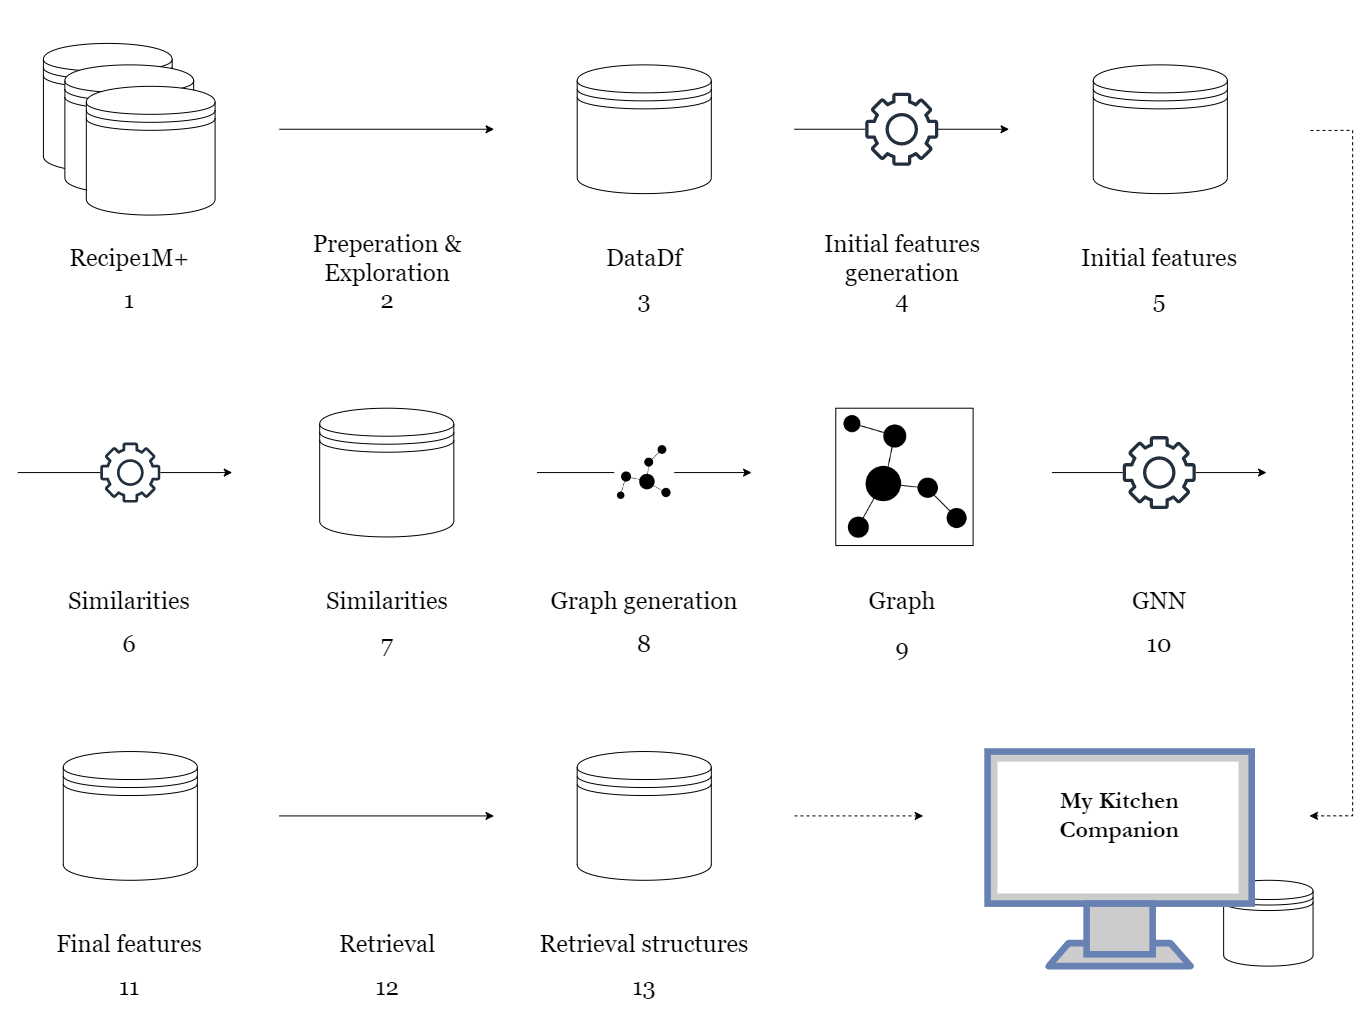
\includegraphics[width=0.7\linewidth]{"D:/Winter23/IIS/096235_Final_project/My kitchen companion/data/others/diagram.png"}
	\caption[s]{Diagram}
	\label{fig:diagram}
\end{figure}
\section{Minimal user evaluation}
We examine the experience of 5 users, Matan's parents Nitay's parents, and Nitay's brother.
All users got it very quick, they understood what they needed to do and what and why the system retrieved. When we asked about their interactive experience, all them answered that the system is very interactive and responds very fast. However some questions were asked. Three of them didn't understand exactly the time and health bar because they were not sure which side is more or less time/health. Two of them said that in the time bar we should have add how much time does the recipe takes and not just more/less time.\\
In addition four of them, said that it could be more helpful if the system would have presented images of the food such that they could have decide if they want this recipe by the look of it.
Moreover two of our users didn't manage to get back to the most relevant recipe after they got down the list and got to less relevant recipes. \\
But after all we think that the users really liked our system and thought that it is very helpful and interactive.
\pagebreak
\section{Summary}
We really enjoyed to implement an end to end system, from gathering the data, analyzing and exploring the data, initial feature engineering, building a learning model and build and design an interactive interface. We learned that it is not that easy to handle and use such big data and that we have to give up some of our in order that the system will work without any problems.
We also learned about some crucial things that the interface must support in order to be helpful and that the work doesn't finished with the learning model. We also learned how important is to let someone else to test your system, because by that, we could hear and learn things that we didn't even think that they are problems.\\\\
If we had more time we would first fix what we were told in the user evaluation. We would add images to the retrieved recipes and change the time and the health bar to be more understandable.
We would try other graph's architectures and we would expand the user's personal zone.
We also want to add even more abstract concepts such as comforting food or home-reminder food or nostalgic one. We also would try to optimize the computation in order to add more data to learn from and that can be retrieved.



\pagebreak
\bibliographystyle{plain}
\bibliography{references}
\end{document}
